\section{Exact Algorithm: {\sf CSM-E}}
\label{sec:exact_algo}
\begin{comment}
A Na\"{\i}ve approach to find the top-$k$ correlated pairs would be to {\bf (1)} first identify
all frequent subgraph patterns based on the minimum support threshold $\Sigma$ (e.g.,
via GRAMI \cite{EASK14}); {\bf (2)} enumerate all their instances in the data graph (e.g.,
via VF3 \cite{CarlettiFSV18}); {\bf (3)} compute correlation for every pair of frequent subgraph patterns;
and finally {\bf (4)} report the top-$k$ correlated pairs among them. However, this baseline method
is inefficient: Since we are interested in finding {\em only} the top-$k$ correlated pairs, computing
correlations for all pairs of frequent subgraph patterns would be expensive and also redundant.
\end{comment}
In this section, we design an {\em exact} and {\em holistic} algorithm, referred to
as {\sf CSM-E} (an abbreviation for Correlated Subgraphs Mining-Exact)
that follows {\em best-first exploration} of
frequent patterns, coupled with an {\em early termination} strategy, to report the top-$k$ correlated
subgraph pairs in a large network.
%
\subsection{Overview}
\label{sec:exact_algo_overview}
%
To find the relevant frequent patterns and the top-$k$ correlated pairs in a
holistic manner, we consider a {\em pattern search tree} $T$, whose $n$-th level
vertices \footnote{{\footnotesize To distinguish the nodes of the pattern search
tree $T$ from those of the data graph $G$, we use the notation ``vertices'' for
the pattern search tree.}} contain $n$-edge frequent subgraphs. In other words,
the first level of the pattern search tree consists of all frequent edges from
the data graph $G$. For any frequent subgraph in the pattern search tree, we use
{\em subscripts to label its nodes according to their discovery order}
\cite{YH02}. Thus, in a frequent subgraph in $T$, $i<j$ indicates that $v_i$ is
discovered before $v_j$. If there is an edge from $v_i$ to $v_j$ with $i<j$,
then it is called a {\em forward edge}; otherwise the edge is denoted as a {\em
backward edge}. We call $v_0$ the root and $v_n$ the rightmost vertex, where $n$
is the number of nodes in that frequent subgraph. The direct path (consisting
of forward edges only) from $v_0$ to $v_n$ is referred to as the {\em rightmost
path}.

To construct $(n+1)$-th layer from the $n$-th layer in the pattern search tree
$T$, a vertex in the $n$-th layer (which is a frequent subgraph, say $P$, from
$G$ having $n$ edges) is augmented with a new edge, and thus we create a new
subgraph, say $C$. We insert $C$ as a vertex in the $(n+1)$-th layer of $T$ if
and only if $C$ is also a frequent subgraph in $G$. We refer to $P$ as a {\em parent
vertex} and $C$ as its {\em child vertex} in $T$. Note that for an $n$-edge
graph, it may have $n$ different ways to be formed from $(n-1)$-edge graphs if
we do not consider isomorphism. The generation of {\em duplicate graphs} is
redundant and could affect the overall efficiency. To reduce the creation of
duplicate graphs, we follow the strategy developed in gSpan \cite{YH02}: {\em A
new edge can only grow from nodes along the rightmost path}. In
particular, {\bf (1)} backward edges can only grow from the rightmost node $v_n$
of $P$, while {\bf (2)} forward edges can grow from nodes on the rightmost path in
$P$. The {\em completeness guarantee} of generating all frequent subgraphs via
the aforementioned {\em rightmost extension} strategy can be found in
\cite{YH02}, and we omit the proof for brevity.

We note that the pattern search tree $T$ is not fully materialized, instead it
is built on demand. For example, gSpan \cite{YH02} explores $T$ in depth-first
manner; whereas in earlier apriori-based approaches (e.g., AGM \cite{IWM00} and
FSG \cite{KK01}) construct $T$ in breadth-first manner. However, we find that
neither depth-first exploration, nor breadth-first exploration is efficient for
our {\bf Top-$k$ Correlated Subgraphs} discovery problem. Rather, we propose a
novel {\em best-first exploration} algorithm, details of which are given in
\S~\ref{sec:bfe}.

Next, when a new frequent pattern $C$ is added in the pattern search tree $T$,
we compute $C$'s correlation with previously explored vertices in $T$ (i.e.,
frequent patterns from $G$ that have been discovered earlier than $C$). In
\S~\ref{sec:replica}, we discuss a memory-efficient data structure,
called $\mathcal{R}$eplica, to find correlation between a pair of frequent
subgraph patterns.

Finally, we employ a {\em priority queue} $\mathcal{Q}$ to store the top-$k$
correlation values (and the corresponding correlated subgraph pairs) found thus
far. In \S~\ref{sec:early_termination}, we further propose an {\em early
termination} strategy to speed up search, while returning the {\em
exact} top-$k$ correlated pairs upon termination.
This completes our algorithm.
%
\subsubsection{Best-First Exploration}
\label{sec:bfe}
%
A pair of subgraph patterns having individual higher support values can be
expected to have higher correlation between them. This is as such subgraph
patterns will have many instances which would likely be closer to each other in
the data graph $G$. Therefore, in the earlier stages of our algorithm, it is
more beneficial to consider patterns with higher support values; it can be
achieved via the best-first exploration of the pattern search tree. In
particular, let us denote by $\mathbb{P}$ the set of frequent patterns currently
in the pattern search tree $T$, whereas we represent by $\mathbb{C}$ the set of
their children that are frequent and also \emph{not} included in $T$. Among
all patterns in $\mathbb{C}$, we pick the one $C^*$ with the maximum support for
inclusion in $T$. We implement $\mathbb{C}$ as another \emph{priority queue} (referred
to as the {\em search queue} in our algorithm) to quickly extract $C^*$ from it.
Formally,
%
\begin{align}
& \mathbb{C}=\{C: \exists P \in T, C \, \text{is }P\text{'s child}, \sigma(C)\ge \Sigma, C \not\in T\} \nonumber & \\
& C^* =\arg\max_{C\in\mathbb{C}}\sigma(C) \nonumber &
\end{align}

If two or more patterns in $\mathbb{C}$ have the same maximum support, we add
one more condition in our best-first exploration: Among them, the pattern with
less number of edges is extracted earlier from $\mathbb{C}$}. This rule coupled
with the downward-closure property of the MNI support ensures that {\em all
subgraphs of $C^*$ must be included in $T$, before $C^*$ is extracted from the
search queue $\mathbb{C}$}.

We notice that unlike gSpan \cite{YH02}, depth-first exploration of the pattern search tree is not optimal in our case since
it identifies many subgraph-supergraph pairs at earlier stages, which are not useful for the {\bf Top-$k$ Correlated
Subgraphs} finding problem. On the other hand, breadth-first exploration is more memory intensive, and based on our
detailed empirical results in \S~\ref{sec:experiments}, it is still inefficient compared to our proposed
best-first exploration strategy.

\spara{Removing duplicates.} While the rightmost extension rules in gSpan
\cite{YH02} reduce the creation of duplicate graphs, it cannot entirely remove
them. To completely eliminate duplicated subgraphs, we further take advantage of
the {\em minimum DFS code} \cite{YH02}: whenever a subgraph $C^*$ is extracted
from $\mathbb{C}$, we compute its minimum DFS code, denoted as $MinDFS(C^*)$. We
also use a hash table $H$ to store all the minimum DFS codes for the vertices
(i.e., frequent subgraphs) already in $T$. When a new subgraph $C^*$ is
extracted, we perform a lookup for $MinDFS(C^*)$ in $H$. If found, then $C^*$
must have been discovered before, since two graphs will have the same minimum
DFS code if and only if they are isomorphic \cite{YH02}, therefore we do not
insert $C^*$ in $T$.
% via VF3 \cite{CarlettiFSV18}

\spara{Removing subgraph-supergraph pairs.} To avoid calculating correlations
between subgraph-supergraph pairs, we check if $C^*$ is a supergraph of already
included frequent patterns in $T$ by performing an explicit subgraph isomorphism
check between $C^*$ and every pattern $Q$ in $T$. Since practically $C^*$ and $Q$ are
small subgraphs and $T$ is also not exceptionally large, we find this to be an
inexpensive operation.
%
\subsubsection{Early Termination Criteria}
\label{sec:early_termination}
%
Our objective is to mine the top-$k$ pairs of correlated (frequent) subgraphs,
and ensure that some other pair of frequent subgraphs cannot have a higher
correlation $(\kappa)$ than any pair in our {\sf Top-$k$} {\em priority queue}
$\mathcal{Q}$. A closer look at Lemma~\ref{lemma:prune} mentioned in
\S~\ref{sec:characteristics} allows us to deduce the following. Consider that
$C^*$ is the current frequent subgraph extracted from $\mathbb{C}$. By
Lemma~\ref{lemma:prune}, $\kappa(C^*,Q,h)\le \sigma(C^*)$, for all frequent
subgraphs $Q$ already in the pattern search tree $T$. Moreover, for any other
pattern $C_1$ that would be added in $T$ after $C^*$,
$\sigma(C_1)\le\sigma(C^*)$ due to best-first exploration thereby resulting in
$\kappa(C_1,Q,h)\le \sigma(C_1) \le \sigma(C^*)$, for all $Q$ in $T$. Hence, if
$\sigma(C^*)$ is lower than the least correlation value ($\kappa$) currently
stored in $\mathcal{Q}$, while $\mathcal{Q}$ being full, we can safely terminate
our search, and report the subgraph pairs in $\mathcal{Q}$ as our exact
solution set.

It is also possible that $k$ correlated pairs do not even exist in the data graph $G$,
given some higher minimum support threshold $\Sigma$ and larger values of $k$. In this case, the {\em priority queue} $\mathcal{Q}$
will never get full, and yet there would not exist any more frequent subgraph to
include in $T$. Thus, we terminate our algorithm.
%
%
\begin{algorithm}[tb!]
{\scriptsize
 \dontprintsemicolon
 \caption{\textsc{Mining Top-$k$ Correlated Pairs}}
 \label{algo:exact}
 \nonl \textbf{Input:} data graph $G=(V,E,L)$, minimum support threshold $\Sigma$,
 distance threshold $h\ge0$, positive integer $k$ \;
 \nonl \textbf{Output:} Top-$k$ pairs of correlated patterns \emph{s.t.} each
 pattern has support $\ge \Sigma$  \;
 Initialize {\sf Pattern Search Tree} $T\leftarrow\ \emptyset$ \;
 Initialize {\sf Search Queue} $\mathbb{C} \leftarrow ${\sf\ Frequent Edges} in $G$\;
 Initialize {\sf Hash Table} $H\leftarrow\ \emptyset$ \; %\COMMENT{stores {\sf Min DFS Codes} of subgraphs in $T$} \;
 Initialize {\sf Priority Queue} $\mathcal{Q}\leftarrow\ \emptyset$ with maximum size $k$ \; %\COMMENT{stores {\sf Top-$k$ Correlated Pairs} found so far} \;
 \While(\tcp*[h]Search){\textup{$\mathbb{C}$ is non-empty}}
 {
   Pattern $C^* \leftarrow$ {\sf Best-First-Pop($\mathbb{C}$)} (\S~\ref{sec:bfe}) \;
   \If {\textup{\textsc{Termination Condition} (\S~\ref{sec:early_termination}) is {\sf True}}}
   {
     Goto Line 19 \;
   }
   \If {\textup{$MinDFS(C^*)  \not\in H$}}
   {
       \lIf {\textup{$\exists \langle Q_1,Q_2 \rangle \in \mathcal{Q}, \kappa(Q_1,Q_2,h)=\sigma(C^*), C^*\succeq Q_1,Q_2$ }}
       {
         Remove $\langle Q_1,Q_2 \rangle$ from $\mathcal{Q}$ \;
       }
       \ForEach{\textup{$Q\in T$}}
       {
         \If {\textup{$Q$ is not a subgraph of $C^*$}}
         {
            Compute correlation $\kappa(C^{*},Q,h)$ (\S~\ref{sec:replica})\;
            Insert $\kappa(Q_1,Q_2,h)$ in $\mathcal{Q}$ (if necessary) \;
         }
       }
       Insert $C^*$ in $T$, $MinDFS(C^*)$ in $H$ \;
      %  Insert
	   \makebox[\linewidth][l]{Find {\sf Children}$(C^*)$ via {\sf Rightmost Extension} (\S~\ref{sec:exact_algo_overview})}\;
	% \makebox[\linewidth][l]{{\sf Children}$(C^*)$ $\leftarrow Extend(C*) {\sf Rightmost Extension} (\S~\ref{sec:exact_algo_overview})}\;
       \ForEach{\textup{{\sf Child}$ \in {\sf Children}(C^*)$}}
       {
         \lIf {\textup{$\sigma$({\sf Child})$\ge\Sigma$}}
         {
           Insert {\sf Child} in $\mathbb{C}$ \;
         }
       }
   }
 }
 \Return {\textup{Top-$k$ correlated pairs currently in $\mathcal{Q}$}}\;}
\end{algorithm}
%

\spara{Removing subgraph pairs with high correlation only due
to a frequent supergraph.} We now turn our attention to the problem of
disregarding subgraph pairs $Q_1$ and $Q_2$
from our top-$k$ priority queue when the pair has high correlation {\em only} because both $Q_1$ and $Q_2$ are
subgraphs of another frequent pattern $C^*$, i.e., $C^* \succeq Q_1$ and $C^* \succeq Q_2$.

In particular, we are concerned when the supergraph $C^*$ of both $Q_1$ and
$Q_2$ has the same support as the correlation between $Q_1$ and $Q_2$, where the
pair $Q_1,Q_2$ is currently in the top-$k$ priority queue $\mathcal{Q}$. Since
$\sigma(C^*)=\kappa(Q_1,Q_2,h)$, and the pair $Q_1,Q_2$ is in $\mathcal{Q}$, the
termination criteria of our algorithm will not be satisfied. Next, to remove the
pair $Q_1,Q_2$ from $\mathcal{Q}$, we incorporate the following procedure in our
mining algorithm: every time a new pattern $C^*$ is extracted from the search
queue $\mathbb{C}$, if the termination criteria is not satisfied, we check if
there exists a correlated pair $Q_1,Q_2$ in $\mathcal{Q}$, such that both $Q_1$
and $Q_2$ are subgraphs of $C^*$ and $\sigma(C^*)=\kappa(Q_1,Q_2,h)$, in
which case we eliminate the pair $Q_1,Q_2$ from $\mathcal{Q}$.

\subsubsection{Putting Everything Together}
\label{sec:exact_description}
%
Our pipeline is described in Algorithm~\ref{algo:exact}.
It begins with finding all frequent edges in data graph $G$,
which are then queued in the search queue $\mathbb{C}$
following a frequency-determined priority ordering (Line 2).
\textit{Search} begins and continues as long as $\mathbb{C}$ contains queued patterns
and the termination condition is unsatisfied (Lines 5-18).
$C^{*}$, selected as the best-first choice
from $\mathbb{C}$, is processed for correlation (\S~\ref{sec:cor_compute}) with every other
previously explored pattern $Q$ in search tree $T$ subject to satisfaction of
constraints described in \S~\ref{sec:bfe}, \ref{sec:early_termination} (Lines 6-13). Top-$k$ priority queue is updated
based on the computed $\kappa$ values (Line 14). $C^{*}$ is then inserted in $T$ and its
minimum {\sf DFS Code} is inserted in $H$ (Line 15), followed by the extension of $C^{*}$ to generate
its \emph{child} patterns. All frequent children of $C^{*}$ are inserted
in $\mathbb{C}$ for future processing and the loop continues (Lines 16-18).
Upon termination, the algorithm returns Top-$k$ pairs of correlated subgraph (Line 19).
%
\subsection{Storing Subgraph Instances: The $\mathbfcal{R}$eplica}
\label{sec:replica}
%
We now focus on the problem of correlation computation between two subgraph patterns
which requires enumerating and finding distances between every pair of instances for
both these patterns. This is memory intensive and computationally demanding due to the
following reasons: {\bf (1)} Storing all instances of all frequent subgraphs discovered so far
can easily overwhelm the memory. We notice that for the frequent
subgraph mining algorithms, e.g., in gSpan \cite{YH02} and GraMi \cite{EASK14},
storing all instances of all discovered frequent patterns is not required.
This illustrates an additional challenge of our problem. {\bf (2)} Many
redundant distance computations could take place: assume two instances
$I_1$ and $I_2$ for patterns $Q_1$ and $Q_2$ respectively, are within $h$-hops
in $G$. Consider a superpattern $Q_3 \succeq Q_1$, and $I_3$, which is extended from $I_1$, is an
instance of $Q_3$. To compute correlation between $Q_3$ and $Q_2$,
verifying the distance between their instance pairs $I_3$ and $I_2$ respectively
is redundant, since
it is guaranteed that they would also be within $h$-hops in $G$.

We solve both these challenges with an efficient data structure, called $\mathcal{R}$eplica
that stores all instances of a subgraph pattern in a compressed manner (\S~\ref{sec:rep_data}).
Our $\mathcal{R}$eplica structure also helps quickly generate instances of a superpattern
extended from a parent pattern (\S~\ref{sec:rep_generate}). Moreover, we design an {\em incremental distance
indexing} method (\S~\ref{sec:index}) that permits deletion of $\mathcal{R}$eplicas of those patterns in $T$
for which all their frequent children patterns (obtained via rightmost extension) have also
been included in $T$. In other words, at any point in our algorithm, we only store $\mathcal{R}$eplicas for the 
following patterns: {\bf (1)} The pattern $C^*$ that is currently extracted from the search queue $\mathcal{Q}$
(Line 6, Algorithm~\ref{algo:exact}), and {\bf (2)} {\em only} those patterns in $T$ for which they have at least one child
in the search queue $\mathbb{C}$. This greatly facilitates in reducing memory footprints 
and redundant distance computations. Finally, we introduce the
correlation computation strategy in \S~\ref{sec:cor_compute}.
%
\subsubsection{$\mathcal{R}$eplica Data Structure}
\label{sec:rep_data}
%
Given the data graph $G$ and a pattern $Q=(V_Q,E_Q,L)$, $\mathcal{R}$eplica$(Q)=(V_{\mathcal{R}(Q)},E_{\mathcal{R}(Q)},L)$ is a subgraph of $G$,
constructed by the {\em graph-union}
\footnote{{\footnotesize The union $\mathcal{G} = \mathcal{G}_1 \cup \mathcal{G}_2$ of graphs $\mathcal{G}_1=(V_1,E_1,L)$
and $\mathcal{G}_2=(V_2,E_2,L)$ is $\mathcal{G} = (V_1\cup V_2, E_1\cup E_2,L)$.}}
of all instances of $Q$ in $G$. Since $\mathcal{R}$eplica$(Q)$ is a subgraph, it is stored as an adjacency list in the memory.

In addition to the aforementioned graph, we store two kinds of node mappings as follows:

\spara{Forward Node Mapping.} $\forall u \in  V_Q$, forward node mapping $Mapping(u,\mathcal{R}\text{eplica}(Q))$
stores all nodes $v\in V_{\mathcal{R}(Q)}$,
such that $v$ is a mapping of $u$ in some instance $I$ of $Q$ within $\mathcal{R}$eplica$(Q)$.

\spara{Inverse Node Mapping.}  $\forall v \in V_{\mathcal{R}(Q)}$, inverse node mapping
$Mapping^{-1}$ $(v, Q)$ stores the set of all $u\in V_Q$ such
that $v\in Mapping(u,\mathcal{R}\text{eplica}(Q))$.

$\mathcal{R}$eplica provides a middle-ground compared to two extreme alternatives: {\bf (1)}
{\em explicitly} store all instances of all generated patterns \cite{KK04}, or {\bf (2)} enumerate all instances
of a pattern whenever required (in runtime) from the {\em large} data graph $G$. In contrast to these alternatives,
the {\em $\mathcal{R}$eplica is economical from both storage and efficiency point of view: it not only avoids
potential memory requirement issues by {\em implicitly} storing
all instances of a pattern, but also lays a robust foundation for carrying out
efficient correlation calculations that we shall discuss in \S~\ref{sec:cor_compute}}.

Note that both forward and inverse node mappings can be deduced from the
$\mathcal{R}$eplica$(Q)$ subgraph via subgraph isomorphism with the pattern $Q$.
However, we explicitly maintain these mappings for computational efficiency:
Forward Node Mapping allows us to readily compute $\sigma(Q)$ and also assists
in $\mathcal{R}$eplica generation, while the Inverse Node Mapping enables us to
quickly prune candidate nodes of $\mathcal{R}$eplica$(Q)$ for matching with a
node in $Q$ while performing isomorphism. The utility of using these mappings
will become apparent in \S~\ref{sec:rep_generate}.
%
\subsubsection{On-Demand Replica Generation for a New Pattern}
\label{sec:rep_generate}
%
\begin{algorithm} [tb!]
 \caption{\textsc{Build Replica for a New Pattern}}
 \label{algo:getreplica}
{\scriptsize
 \dontprintsemicolon
 \nonl \textbf{Input:} data graph $G=(V,E,L)$, parent
 pattern $Q=(V_Q,E_Q,$ $L)$, $\mathcal{R}$eplica$(Q)=(V_{\mathcal{R}(Q)}$,
 $E_{\mathcal{R}(Q)}$, $L)$, child pattern $R=(V_R$, $E_R$, $L)$, extending node:
 $u\in V_Q$, extending edge: $(u,v) \in E_R$ \;
\nonl \textbf{Output:} $\mathcal{R}$eplica$(R)$ \;
	\vspace{0.3mm}
	$DFS\ List(Q)\leftarrow$ get edge list via rooted DFS in $Q$ with $u$ as root \;
	Initialize $instance \leftarrow \emptyset, $ $ \mathbb{I} \leftarrow \emptyset$\;
	\ForEach{ $u' \in Mapping(u,\ \mathcal{R}$\textup{eplica}$(Q))$}
	{
		$instance.{\sf add}(u\mapsto u')$\;
		\ForEach{\textup{edge} $(u',v')\in E_G$ \textup{that maps to the extending edge} $(u,v)\in E_R$}
		{
			$instance.{\sf add}(v\mapsto v')$\;
	        $\mathbb{I}\leftarrow$ \textsc{FindAllInstances($G$, $Q$, $\mathcal{R}eplica(Q)$, $R$,
	        $DFS\ List(Q)$, $instance$, $\mathbb{I}$)}\;
			\textsc{UpdateReplica($R$, $\mathcal{R}eplica(R)$, $\mathbb{I}$)}\;
			% $instance\leftarrow instance \setminus \{(v,v')\}$\;
			$instance.{\sf delete}(v\mapsto v')$\;
		}
		% $instance\leftarrow instance \setminus \{(u,u')\}$\;
		$instance.{\sf delete}(u\mapsto u')$\;
	}	
	\Return{$\mathcal{R}$\textup{eplica}$(R)$}\;}
\end{algorithm}
%
\vspace{-2mm}
\begin{algorithm}[tb!]
 \caption{\textsc{FindAllInstances:Exact Method}}
 \label{algo:findallinstances}
{\scriptsize
 \dontprintsemicolon
 \nonl \textbf{Input:} data graph $G=(V,E,L)$, parent
 pattern $Q=(V_Q,E_Q,$ $L)$, $\mathcal{R}$eplica$(Q)=(V_{\mathcal{R}(Q)}$,
 $E_{\mathcal{R}(Q)}$, $L)$, child pattern $R=(V_R$, $E_R$, $L)$,
    $DFS\ List(Q)$, partial isomorphism of $R$: $instance$, $\mathbb{I}$\;
\nonl \textbf{Output:} $\mathbb{I}: $ set of all instances of $R$ in $G$ consistent with input partial isomorphism $instance$\;
	\uIf{$instance$ \textup{is} {\sf Found}}
	{
		\Return{$\{instance\}$}
	}
	\Else
	{
		$e=(p,c)\leftarrow$ \textsc{NextQueryEdge($DFS\ List(Q)$)}\;
		$v' \leftarrow instance(p)$\;
		\uIf{$e$ \textup{is a} {\sf backward edge}}
		{
			\uIf{\textup{an edge} $(v',instance(c))$ \textup{exists in} $E_{\mathcal{R}(Q)}$}
			{
				$\mathbb{I} \leftarrow \mathbb{I}\ \cup$ \textsc{FindAllInstances({$G$}, $Q$, $\mathcal{R}eplica(Q)$, $R$, $DFS\ List(Q)$, $instance$, $\mathbb{I}$)}\;
			}
			\Else{\Return $\emptyset$}
		}
		% (\tcp*[h]{{$e$ is a forward edge}})
		\Else{
		$P_{c} \leftarrow$ \textsc{FilterCandidates($v'$, $c$, $Q$, $\mathcal{R}eplica(Q)$)}\;
		\ForEach{$w' \in P_{c}$ s.t. \textup{$w'$ is not matched in} $instance$}
		{
		%   $instance \leftarrow instance \cup \{(c,w')\}$\;
			$instance.{\sf add}(c\mapsto w')$\;
			$\mathbb{I} \leftarrow \mathbb{I}\ \cup$ \textsc{FindAllInstances({$G$}, $Q$, $\mathcal{R}eplica(Q)$, $R$, $DFS\ List(Q)$, $instance$, $\mathbb{I}$)}\;
		% $instance \leftarrow instance \setminus \{(c,w')\}$\;
			$instance.{\sf delete}(c\mapsto w')$\;
		  }}
		\Return{$\mathbb{I}$}\;
	}}
\end{algorithm}
%
%
We create $\mathcal{R}$eplicas in an incremental manner: given $\mathcal{R}$eplica$(Q)$ of a parent
pattern $Q$, we generate $\mathcal{R}$eplica$(R)$ of its child pattern $R$. Our exact approach for
replica extension is given in Algorithm~\ref{algo:getreplica}, which essentially describes a backtracking
procedure for subgraph isomorphism similar to the {\em Ullman's algorithm} \cite{U76}.


Algorithm \ref{algo:getreplica} begins with a depth-first search ({\sf DFS}) procedure (Line 1)
executed on parent $Q$, selecting $u\in V_{Q}$ at which the
\emph{extending edge} $(u,v)$ is grown as the \emph{root}. We call $u$ the
\textit{extending node}. Both forward and backward edges encountered in the {\sf DFS}
starting at $u$ are recorded in an ordered list called the \emph{DFS List},
which guides the isomorphism performed subsequently. For every mapping $u'$ of
$u$ in $\mathcal{R}$eplica$(Q)$, the algorithm attempts to enumerate all
instances of child $R$ in $G$ fixing $u\mapsto u'$ (Lines 3-10). It does so by matching $v$
next, the newly extended node to all nodes $v'\in V$ adjacent to $u'$,
such that edge $(u',v')\in E$ is a valid mapping for $(u,v)\in E_{R}$ (Lines 5-6). It
then invokes \textsc{FindAllInstances} (Algorithm \ref{algo:findallinstances})
which uses $\mathcal{R}$eplica$(Q)$ to find every instance of $R$ such that
$u\mapsto u'$ and $v\mapsto v'$ (Line 7).

Algorithm \ref{algo:findallinstances}, as invoked above, recursively enumerates all instances
of $R$ in a depth-first manner following \emph{DFS List(Q)}. In the general case (Lines 4-17), the algorithm
begins by invoking \textsc{NextQueryEdge} which returns one edge at a time from
$E_{Q}$ in the order of \emph{DFS List(Q)}. Edge $e=(p,c)$, thus returned, connects
nodes $p,c \in V_Q$ such that $c$ is the pattern node to be matched next; $p$ is already
matched to $v' \in V_{\mathcal{R}(Q)}$. (The first call to
Algorithm \ref{algo:findallinstances} in every iteration of the inner loop in
Algorithm \ref{algo:getreplica} always has $p$ matched with $u'$).
If, however, $e$ is a backward edge, $c$ is already matched in which case the
algorithm checks whether an edge exists in $\mathcal{R}$eplica$(Q)$
connecting $v'$ and $instance(c)$: if it does exist, it proceeds with the
search for the next node matching, but returns unsuccessfully if it does not. If
$e$ is a forward edge, the algorithm calls \textsc{FilterCandidates} to compute the candidates set $P_c$ for storing
all nodes $w'\in V_{\mathcal{R}(Q)}$ for matching $c$ such that:
\textbf{(1)} $w'$ is a neighbor of $v'$ in $\mathcal{R}$eplica(Q); \textbf{(2)}
$c$ exists in the Inverse node mapping set for $w'$ in $\mathcal{R}$eplica(Q). That
is,
%$\forall$ $w' \in P_{c}$,
$c\in Mapping^{-1}(w', Q)$;
%\textbf{(3)} Edge label of $(v',w')\in E_{\mathcal{R}(Q)}$ matches that of $(p,c)\in E_Q$.
Next, for every node $w' \in P_{c}$ such that $w'$ has not already been matched in the
current \textit{instance}, the algorithm attempts the match $c\mapsto w'$ in \textit{instance}
and recursively calls \textsc{FindAllInstances} to match
remaining pattern nodes following the edges in \textit{DFS List}. \textit{Base
case} (Lines 1-2) occurs when the algorithm finds an \textit{instance} of $R$,
which it simply returns.

The set of all instances $\mathbb{I}$ thus found is returned by Algorithm \ref{algo:findallinstances} (Line 17) and is recorded by
Algorithm \ref{algo:getreplica}. In \textsc{UpdateReplica} (Algorithm \ref{algo:getreplica}, Line 8), the algorithm
updates $\mathcal{R}$eplica$(R)$ by performing a graph union with all instances in $\mathbb{I}$. It also updates the
\textit{Mappings} and \textit{Mappings$^{-1}$} indices to record new mappings found for every $instance$ in $\mathbb{I}$.
%
%This $\mathcal{R}$eplica-based instance storage strategy not only builds a foundation for an
%efficient correlation calculations, but also benefits the MNI support counting in
%the single large graph since we can directly get $\sigma(R)$ by counting all the sizes of the $Mapping(v)$, $v\in
%V_Q$.
%
%
%
\begin{figure}[t]
	\captionsetup{textfont=bf,font=small}
	\captionsetup[subfigure]{font=small, skip=-1pt}
	\begin{subfigure}[b]{0.5\textwidth}
		\centering
		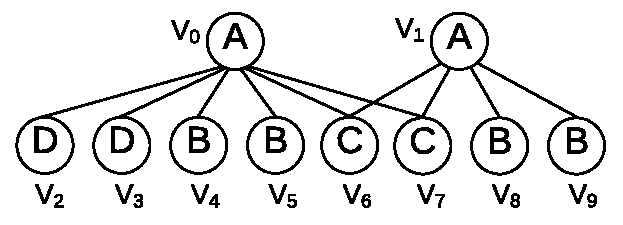
\includegraphics[scale=0.5]{img_ex/G.pdf}\hspace*{2.5em}
		\caption{data graph $G$}
		\label{fig:exactG}
	\end{subfigure}%

    \begin{subfigure}[b]{0.15\textwidth}
            % \centering
            \hspace{4mm}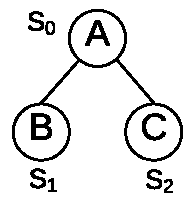
\includegraphics[scale=0.5]{img_ex/patternQ.pdf}
            \caption{Parent $Q$}
			\label{fig:exact-Q}
    \end{subfigure}%
    \hspace*{\fill}
    % \captionsetup[subfigure]{labelfont=bf,textfont=normalfont,singlelinecheck=on,justification=raggedright, skip=-5pt}
	\begin{subfigure}[b]{0.3\textwidth}
            % \centering
            \hspace{-2.5mm}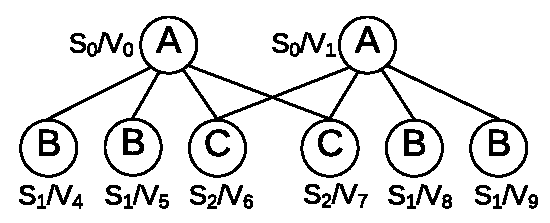
\includegraphics[scale=0.5]{img_ex/replicaQ.pdf}
            \caption{$\mathcal{R}$eplica$(Q)$}
			\label{fig:exact-REPQ}
	\end{subfigure}

	% \captionsetup[subfigure]{skip=-2pt}
	\begin{subfigure}[b]{0.15\textwidth}
		% \centering
		\hspace{4mm}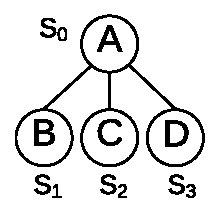
\includegraphics[scale=0.5]{img_ex/patternR.pdf}
		\caption{Child $R$}
		\label{fig:exact-R}
	\end{subfigure}%
	\hspace*{\fill}
	\begin{subfigure}[b]{0.3\textwidth}
		% \centering
		\hspace{0mm}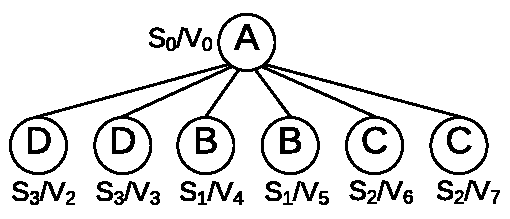
\includegraphics[scale=0.5]{img_ex/replicaR.pdf}
		\vspace{-0.25mm}
		% \vspace{-1.3\baselineskip} %not needed because figures are aligned
		% naturally unline above case
		\caption{$\mathcal{R}$eplica$(R)$}
		\label{fig:exact-REPR}
	\end{subfigure}
	% \captionsetup[figure]{skip=200pt}
    % \vspace{-1.75\baselineskip}
	\caption{$\mathcal{R}$eplica generation for a new subgraph pattern}
	\label{fig:exact-EX}
	% \vspace{0.15\baselineskip}
\end{figure}
%
%
\begin{exple}
Initially, $Q$ and $\mathcal{R}$eplica$(Q)$ are shown in Figs. \ref{fig:exact-Q}
and \ref{fig:exact-REPQ}, respectively. Child $R$, extended from $Q$ at
\emph{extending node} $s_0$ using the \emph{extending edge} $(s_0, s_3)$ is
given in Figure \ref{fig:exact-R}. Assume \emph{DFS List} for \emph{DFS}
starting at $s_0$ records edges $(s_0, s_1)$ and $(s_0, s_2)$ in that order. To
construct $\mathcal{R}$eplica$(R)$, the algorithm iterates over
$Mapping(s_0,\mathcal{R}$eplica$(Q))$, i.e. set $\{v_0, v_1\}$. With $s_0\mapsto
v_0$, the algorithm then considers vertices in $G$ (Fig. \ref{fig:exactG}) for
matching $s_3$. Thus, for each of $s_3\mapsto \{v_2, v_3\}$, the algorithm makes
recursive invocations to map $s_1$ and $s_2$ following the \emph{DFS List}
thus successfully enumerating instances. With $s_0\mapsto v_1$ however, no
mappings for matching $s_3$ exist. Graph union of all instances of $R$ thus
enumerated results in $\mathcal{R}$eplica$(R)$ depicted in Fig. \ref{fig:exact-REPR}.
% Assume, $(V_0, V_6), (V_0, V_7)\in E(G)$ map to $(A, D)$; but no such
% mapping edges exist incident to $V_1$ in $G$. All instances of $R$ thus found
% would result in $\mathcal{R}$eplica$(R)$ depicted in Figure \ref{fig:exactrepr}.
%
\end{exple}
%
\subsubsection{Indexing to Facilitate $\mathcal{R}$eplica Deletion of Old Patterns}
\label{sec:index}
%
We build and maintain two distance-based indexes, which permit us deleting $\mathcal{R}$eplicas of old
patterns once all their frequent children patterns (via rightmost extension) have been 
included in the pattern search tree $T$.

% \squishlist
\spara{\bf Proximity Nodes.} For each frequent node $u$ in data graph $G$, we
store proximity nodes of $u$ that are also frequent, denoted as $CorV(u)$: for
each node $v\in CorV(u)$, it holds that $d(u,v)\le h$.
% \squishend
% \squishlist

\spara{\bf Proximity Patterns.} For each frequent node $u$ in $G$, we store
patterns that are already included in $T$ and are within distance $h$ from
$u$. This is denoted as $CorP(u)$. For each pattern $Q\in CorP(u)$, {\bf (1)}
$Q\in T$, and {\bf (2)} given the instance-groups
$\mathbb{I'}=\{I'_1,I'_2,\ldots,I'_{\sigma(Q)}\}$ of $Q$, $\exists I'\in
\mathbb{I'}$, $\exists v\in I'$, it holds that $d(u,v)\le h$.
% \squishend

The {\em proximity nodes index} ($CorV$) is constructed before our mining
process starts, while the {\em proximity patterns index} ($CorP$) is updated
incrementally every time a new pattern $Q$ is inserted in the pattern search
tree $T$. The details of $CorP$ maintenance will be discussed in
\S~\ref{sec:cor_compute}. Since we already have $h$-hop proximity information
about all existing patterns in $T$, it allows us to delete their $\mathcal{R}$eplica
structures, thereby reducing the memory footprint of our technique.
%
%
\subsubsection{Correlation Computation}
\label{sec:cor_compute}
%
We recall that when a pattern $C$ is extracted from the search queue $\mathcal{Q}$, its
correlation is calculated with every pattern already in the pattern search tree $T$.
In the following, we focus on the computation of correlation $\kappa(C,Q,h)$ between $C$ and some $Q\in T$.
Due to our best-first exploration strategy, $\sigma(C)\le\sigma(Q)$, thus we need to verify
for every instance-group $I'$ of $C$, if there is some instance-group of $Q$ within distance $h$.

First, to find all instance-groups of $C$, our novel data structure $\mathcal{R}$eplica$(C)$ would be
immediately useful: Forward node mapping allows us to readily compute the MNI support of $C$, and the
node $v$ in $C$ having the minimum MNI support. For every $u \in Mapping(v,\mathcal{R}\text{eplica}(C))$,
we enumerate from $\mathcal{R}$eplica$(C)$ all instances of $C$ having $u$ (Algorithm~\ref{algo:findallinstances}).
This generates the instance-group of $C$ containing $u$. In this way, one can also efficiently enumerate all instance-groups
of $C$.

Given an instance-group $I'$ of $C$, we find if any instance-group of $Q$ is  within distance $h$ from $I'$ as demonstrated below.
Consider $CorP(w)$ for all node $w \in I'$. If $\cup_{w \in I'} CorP(w)$ contains $Q$, this essentially indicates that
there is some instance-group of $Q$ within distance $h$ from $I'$.
Ultimately, we count, out of all $\sigma(C)$ instance-groups
of $C$, how many of them are close to at least one instance-group of $Q$.
This count is reported as the correlation $\kappa(C,Q,h)$.
In this way, our {\em proximity nodes index} ($CorP$)
aids in efficient correlation computation.

\spara{Incrementally Updating Proximity Patterns Index.} Finally,
we incrementally update the $CorP$ index as follows. If $CorV(w)$ contains $u$ for some $w\in I'$, we include
the new pattern $C$ in $CorP(u)$. Thus, we also ensure that at any point in our algorithm, $CorP(u)$ would
contain all patterns in $T$ which are within distance $h$ from $u$.
%
%
\subsection{Complexity Analysis}
\label{sec:complexity_exact}
%
For simplicity, we use the notations below:
The data graph $G$ has $n$ nodes and $m$ edges,
among them $n_f$ nodes and $m_f$ edges are frequent based on the input
minimum support threshold. We denote by $n_h$ and $m_h$ the maximum number
of nodes and edges in the $h$-hop of a node in $G$. The pattern search tree
$T$ has at most $n_T$ vertices, with $n'_T$ vertices having at least one frequent child in the search queue $\mathcal{C}$, during the execution of our algorithm. Let the maximum number of nodes and
edges in a pattern $Q$ mined by our method be $n_Q$ and $m_Q$, and those in a replica be
$n_{\mathcal{R}}$ and $m_{\mathcal{R}}$, respectively. Finally,
also assume that the maximum size of the forward node mapping set be $M$
for some node in a frequent pattern mined by our algorithm.
%
\subsubsection{Time Complexity}
We start with the complexity analysis of {\em replica creation} for a new pattern $Q$ (\S~\ref{sec:rep_generate}).
For every mapping of the {\em extending edge} in $G$, we enumerate all possible
instances of $Q$ using the replica subgraph of its parent pattern. There can be $\bigO(m)$
matches for the extending edge, whereas the complexity of enumerating all possible
instances of $Q$ using the parent's replica is bounded by $\bigO(M^{n_Q})$. Hence,
the time complexity of building the replica of $Q$ is $\bigO(mM^{n_Q})$.

The creation of  {\em proximity nodes index} (\S~\ref{sec:index})
requires $h$-hop BFS from every frequent node in $G$,
and hence it has total time complexity: $\bigO(n_f(n_h+m_h))$. In contrast, whenever a new frequent
pattern is mined, one requires updating the {\em proximity patterns index}. This is performed
by traversing every node in the replica of the new pattern, and then finding their $h$-hop frequent
nodes using the proximity nodes index --- this has time complexity $\bigO(n_{\mathcal{R}}n_f)$. Since the pattern search tree
$T$ has at most $n_T$ vertices, total time complexity due to updating of proximity patterns index is
given by $\bigO(n_{\mathcal{R}} n_f n_T)$.

Correlation computation (\S~\ref{sec:cor_compute}) between the new pattern $Q$ extracted from the search queue $\mathbb{C}$
and an existing pattern in $T$ is essentially bounded by the complexity of enumerating all instances of $Q$ in its replica, i.e., $\bigO(M^{n_Q})$.
Since $T$ has at most $n_T$ patterns, one performs $\bigO(n_T^2)$ correlation computations, which has time
complexity $\bigO(n_T^2 M^{n_Q})$.

Considering all above, the time complexity of our exact algorithm, {\sf CSM-E}
\footnote{{\footnotesize We neglected times required for finding the best pattern
from search queue $\mathbb{C}$, verifying its subgraph relationships
with existing patterns in $T$, and computing its rightmost extensions,
due to relatively smaller sizes of frequent patterns mined by our algorithm
while finding the top-$k$ correlated pairs.}} is:
$\bigO(M^{n_Q}(n_T^2+m)+n_{\mathcal{R}}n_fn_T+n_f(n_h+m_h))$. Notice that
{\em we enumerate all instances of a pattern using its replica
(or, the replica of its parent), thereby significantly improving the efficiency in comparison with
na\"{\i}vely enumerating all instances over the entire data graph $G$}. Nevertheless, an exact enumeration of all instances,
as given in Algorithm~\ref{algo:findallinstances}, is still expensive when the replica size is too large
(thereby larger $M$). In \S~\ref{sec:approx_algo}, we shall introduce an approximate method for instances enumeration,
which further improves the efficiency, without significantly affecting the accuracy of our solution.
%
\subsubsection{Space Complexity}
The space complexity is bounded by the {\em replica size} and the {\em size of our index sets}: {\em forward node mapping}
and {\em inverse node mapping}, as well as {\em proximity nodes} and {\em proximity patterns indexes}.
Since we only store the replica of $\bigO(n'_T+1)$ patterns, this requires $\bigO((n_{\mathcal{R}}+m_{\mathcal{R}})n'_T)$ space.
Both forward and inverse node mappings for a pattern $Q$ has size $\bigO(n_QM)$. Finally, proximity nodes
and proximity patterns indexes require $\bigO(n_f^2)$ and $\bigO(n_fn_T)$ space, respectively.  Hence, the overall
space complexity is given by: $\bigO((n_{\mathcal{R}}+m_{\mathcal{R}}+n_QM)n'_T+n_f^2+n_fn_T)$. 


